
\section{System}\todo[inline]{Lukas}
Die Benutzung von \textit{MArC} ist in der dem Programm mitgelieferten ReadMe-Datei beschrieben. Darin wird erklärt, welche Hard- und Software komponenten erforderlich sind, wie das System gestartet und kalibriert wird. Des weiteren enthält die ReadMe eine Übersicht über die enthaltenen Quellcode-Dateien.
\subsection{Aufbau}\label{sec:Aufbau}\todo[inline]{Lukas und Vera}
\begin{figure}[H]
	\centering
	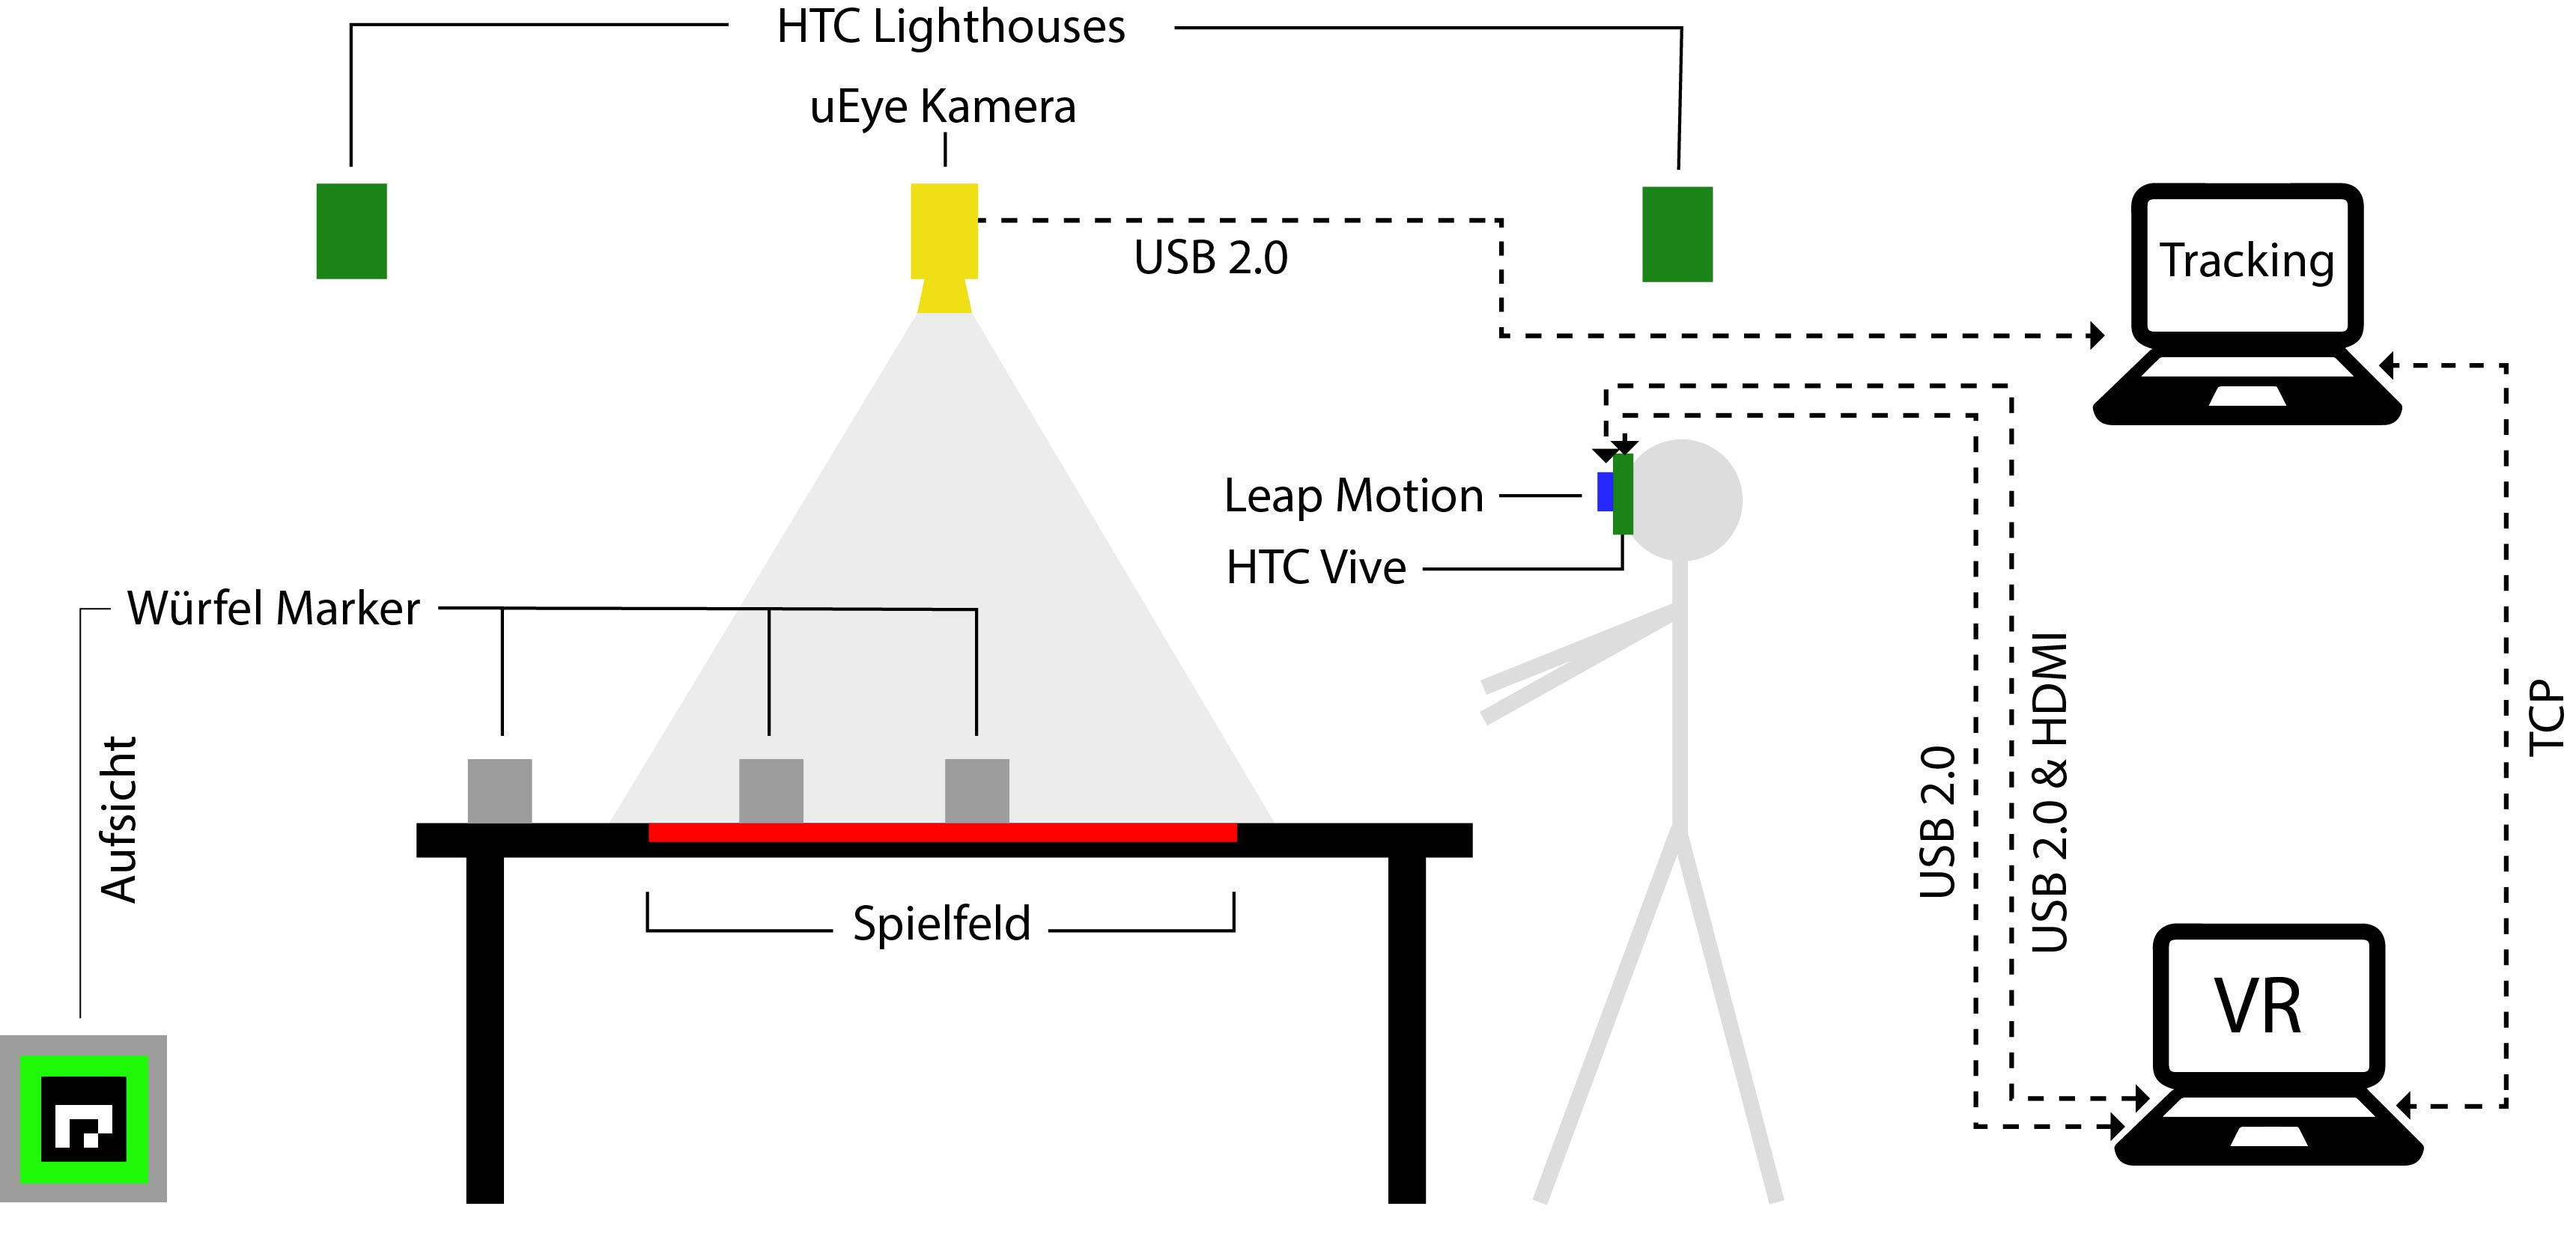
\includegraphics[width=\textwidth]{Bilder/Aufbau_MArC.jpg}
	\caption{Aufbau des \textit{MArC} System.}
	\label{fig:AufbauMarc}
\end{figure}

\begin{figure}[H]
	\centering
	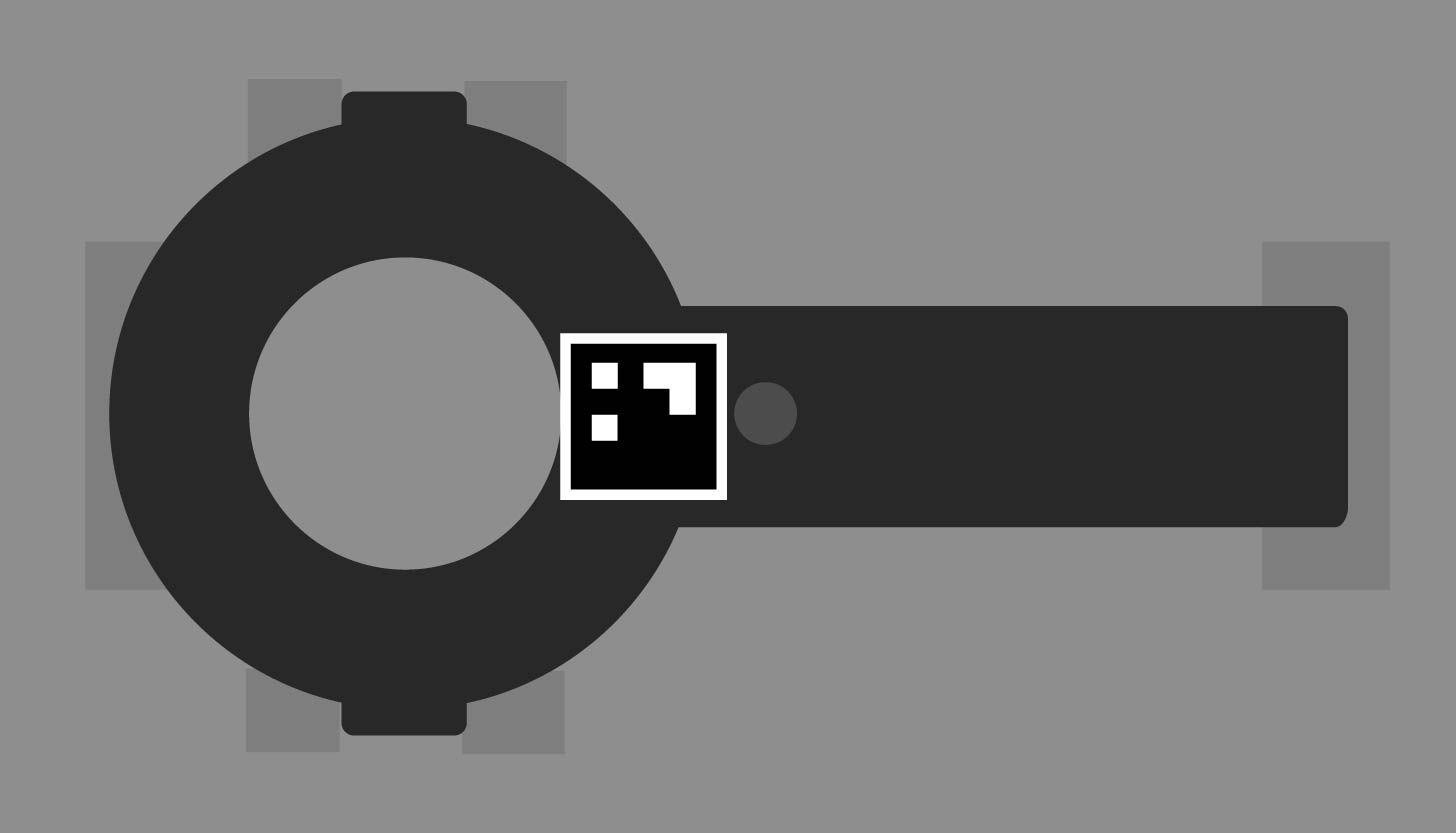
\includegraphics[width=4in]{Bilder/CalibController.jpg}
	\caption{Kalibrierungscontroller des \textit{MArC} System mit ArUco Marker.}
	\label{fig:KontrollerMarc}
\end{figure}

\subsection{Systemvorraussetzung}\todo[inline]{Lukas}
\subsection{Starten des Systems}\todo[inline]{Lukas}
Nachdem sichergestellt wurde, dass alle in der ReadMe-Datei beschriebenen Voraussetzungen bestehen, kann das System gestartet werden, indem zunächst die Tracking-Anwendung (auf dem einen Computer) und anschließend die aus Unity heraus erstellte Anwendung (auf dem anderen Computer) gestartet wird. Auf letzterem Computer beginnt darauffolgend die Menüführung, welche in \ref{sec:menu} beschrieben ist. 
\subsection{Menüführung}\label{sec:menu}\todo[inline]{Lukas}
Die Menüführung dient dazu, den Benutzer durch alle notwendigen Schritte zu leiten, die vor dem Starten der eigentlichen Simulation erforderlich sind. Im nachfolgenden Abschnitt~\ref{sec:menus} werden alle verfügbaren Menüs der Anwendung aufgelistet und kurz beschrieben, während im Abschnitt~\ref{sec:menuAblauf} der Ablauf der Menüführung erläutert wird.

\subsubsection{Menüs}\label{sec:menus}\todo[inline]{Lukas}
Die folgenden Menüs sind Bestandteil der Menüführung:\todo[inline]{Screenshots der Menüs einfügen?}\todo[inline]{Laura}
\begin{description}
	\item[\texttt{CalibDone}:] Wird aufgerufen, wenn die Kalibrierung des Arbeitsbereichs abgeschlossen ist. Es informiert den Benutzer, dass die Kalibrierung erfolgreich war und der Vorgang fortgesetzt werden kann.
	\item[\texttt{CalibrateOrNot}:] Erscheint nach dem Verlassen des \texttt{Welcome}-Menüs und erlaubt dem Benutzer eine Kalibrierung durchzuführen oder eine bereits durchgeführte Kalibrierung zu laden.
	\item[\texttt{ControllerNotFound}:] Warnt den Benutzer nach dem Starten der Kalibrierung, dass der HTC Vive Controller, welcher für die Kalibrierung benötigt wird, nicht eingeschaltet ist. Während das Menü angezeigt wird, kann der Benutzer den Controller einschalten und anschließend auf \texttt{Continue} klicken.
	\item[\texttt{doPlaneCalibInVS}:] Dient dem Benutzer als Anleitung für die Durchführung der Arbeitsbereich-Kalibrierung. Diese wird in \ref{sec:planeCalib} genauer beschrieben.
	\item[\texttt{doPoseCalibInVS}:] Dient dem Benutzer als Anleitung für die Durchführung der Kamera-Kalibrierung. Diese wird in \ref{sec:camCalib} genauer beschrieben.
	\item[\texttt{SelectCalibrationTarget}:] Erlaubt die Auswahl der Art der Kalibrierung. Es kann hier entweder nur der Arbeitsbereich oder sowohl der Arbeitsbereich, als auch die Kamera kalibriert werden. Die Kalibrierung ist näher in \ref{sec:calib} beschrieben.
	\item[\texttt{SetScale}:] Stellt das letzte Menü vor dem Starten der Simulation dar. In diesem kann der Benutzer den Maßstab der Gebäudesimulation einstellen und anschließend die Simulation starten.
	\item[\texttt{SocketNotReady}:] Warnt den Benutzer nach dem Verlassen des \texttt{Welcome}-Menüs, dass die Netzwerkverbindung zum Computer, auf dem die Tracking-Anwendung ausgeführt wird, nicht bereit ist. Nach Bestätigung dieses Hinweises durch einen Klick auf \texttt{Continue}, kehrt der Benutzer zum \texttt{Welcome}-Menü zurück. Anschließend kann der Vorgang fortgesetzt werden, wenn die Netzwerkverbindung hergestellt wurde. Andernfalls erscheint wieder \texttt{SocketNotReady}.
	\item[\texttt{Welcome}:] Erscheint als erstes Menü. Hier erhält der Nutzer eine kurze Information darüber, wie die Anwendung heißt und wozu sie dient.
\end{description}


\subsubsection{Ablauf der Menüführung}\label{sec:menuAblauf}\todo[inline]{Lukas}
Der Ablauf der Menüführung von \textit{MArC} ist in Abbildung~\ref{fig:menuFlow} dargestellt. Die einzelnen Menüs sind bereits in~\ref{sec:menus} beschrieben worden.

\begin{figure}[htbp]
	\centering
	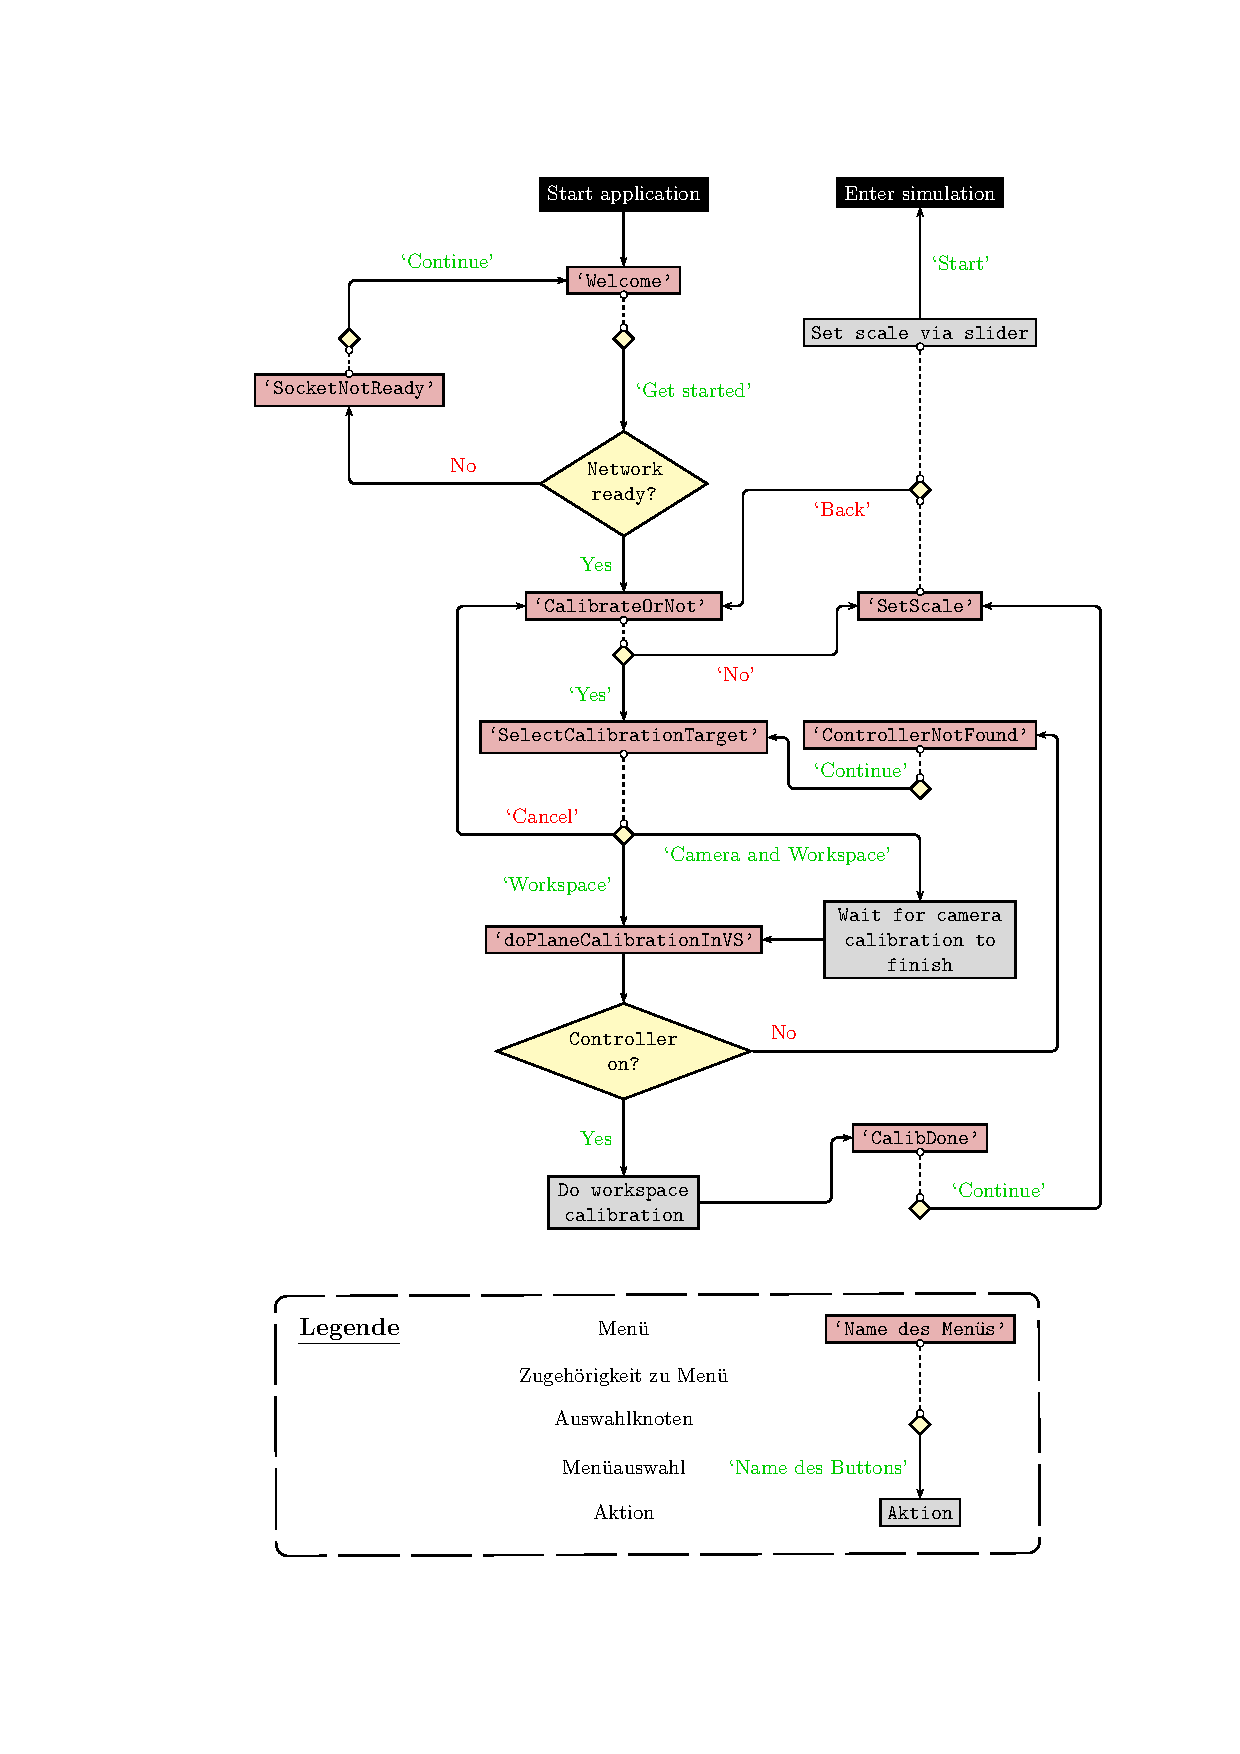
\includegraphics[scale=.9, trim=5.5cm 2.5cm 3.5cm 2.5cm]{kapitel/system/MP_Menu_Flowchart.pdf}
	\caption{Flussdiagramm der Menüführung.}
	\label{fig:menuFlow}
\end{figure}

Nach dem Starten der Anwendung wird zunächst das Menü \texttt{Welcome} angezeigt. Dieses enthält nur einen Button \textit{Get started}. Sobald dieser gedrückt wird, prüft die Anwendung, ob eine Netzwerkverbindung zu dem Computer mit der Tracking-Anwendung besteht. Sollte dies nicht der Fall sein, wird das Menü \texttt{Socket\-Not\-Ready} angezeigt. Dieses verlässt der Benutzer über einen Klick auf \texttt{Continue}, anschließend wird erneut das Menu \texttt{Welcome} angezeigt. Wenn zu diesem Zeitpunkt die Netzwerkverbindung korrekt hergestellt wurde, gelangt der Benutzer zum Menü \texttt{Calibrate\-Or\-Not}, anderenfalls wird wiederholt \texttt{Socket\-Not\-Ready} angezeigt.

In \texttt{CalibrateOrNot} hat der Benutzer die Auswahl zwischen den Schaltflächen \textit{Yes} und \textit{No}. Bei einem Klick auf \textit{Yes} wird anschließend \texttt{Select\-Calibration\-Target} angezeigt, bei einem Klick auf \textit{No} lädt das System eine zuvor durchgeführte Kalibrierung und das Menü \texttt{Set\-Scale} wird geöffnet.

\texttt{Select\-Calibration\-Target} stellt den Benutzer vor die Wahl entweder nur den Arbeitsbereich (\textit{Work\-space}) oder sowohl den Arbeitsbereich als auch die Kamera zu kalibrieren (\textit{Camera and Workspace}). Außerdem besteht die Möglichkeit über \textit{Cancel} zum Menü \texttt{Calibrate\-Or\-Not} zurückzukehren.

Wählt der Benutzer \textit{Camera and Workspace} in \texttt{Select\-Calibration\-Target} aus, so informiert die Anwendung die Tracking-Anwendung auf dem anderen Computer und wartet anschließend darauf, dass von dort die Bestätigung gesendet wird, dass die Kamerakalibrierung abgeschlossen ist. Anschließend wird das Menü \texttt{doPlane\-Calibration\-InVS} angezeigt, welches auch aufgerufen wird, wenn der Benutzer \textit{Work\-space} in \texttt{Select\-Calibration\-Target} wählt.

Im Menü \texttt{doPlane\-Calibration\-InVS} wird zunächst geprüft, ob der für die Kalibrierung notwendige HTC Vive Controller eingeschaltet ist. Sollte dies nicht der Fall sein, wird \texttt{Controller\-Not\-Found} aufgerufen. Dieses kann mit einem Klick auf \textit{Continue} verlassen werden, woraufhin wieder \texttt{Select\-Calibration\-Target} angezeigt wird.\\
Sofern der HTC Vive Controller beim Aufruf von \texttt{doPlane\-Calibration\-InVS} eingeschaltet ist, wird nach Durchführung der Kalibrierung des Arbeitsbereichs das Menü \texttt{CalibDone} angezeigt.

\texttt{Calib\-Done} kann über einen Klick auf \textit{Continue} verlassen werden und führt den Nutzer anschließend zu \texttt{SetScale}. Aus diesem Menü kann über den Button \textit{Back} entweder zu \texttt{CalibrateOrNot} zurückgekehrt oder die Simulation mit dem im Menü über den Slider eingestellten Maßstab gestartet werden.

\subsection{Toogle}\todo[inline]{Paul}

\subsection{Kontex Menü}\todo[inline]{Laura und Lukas}
\subsubsection{Menüführung}\todo[inline]{Laura}
\subsubsection{Architektur Berechnung}\todo[inline]{Laura}


\subsection{Table Menü}\todo[inline]{Paul}
\subsubsection{Szenen Management}\todo[inline]{Paul}
\subsubsection{Match Modus}\todo[inline]{Paul}

\subsection{Tracking Algorithmus} \label{sec:Tracking}\todo[inline]{Vera}
\subsubsection{Green Keying}\todo[inline]{Vera}
\subsubsection{ArUco Marker Tracking}\todo[inline]{Vera}
\subsubsection{Marker Objekt}\todo[inline]{Vera}
\subsubsection{Zuordnung der Identitäten}\todo[inline]{Vera}



\subsection{Kalibrierung}\label{sec:calib}\todo[inline]{Laura}
Um das Ziel von \textit{MArC} zu erreichen, an den Positionen der Aluminiumwürfel im Arbeitsbereich in der virtuellen Realität von Unity gerenderte Würfel darzustellen, muss das System kalibriert werden. Die Kalibrierung hat zum Ziel, eine Koordinatentransformation zu finden, die Positionen im Kamera-Koordinatensystem in das Unity-Koordinatensystem transformiert.

Zu diesem Zweck muss eine zweistufige Kalibrierung durchgeführt werden. Zunächst sorgt die Kamerakalibrierung dafür, dass Bildkoordinaten auf dem Sensor der Kamera in das 3D-Kamera-Koordinatensystem transformiert werden. Dafür wird sich einiger OpenCV-Funktionen in Verbindung mit AruCo-Markern bedient. Dieser Vorgang wird nachfolgend in~\ref{sec:camCalib} genauer beschrieben.\\
Der nächste Schritt, die Kalibrierung des Arbeitsbereichs, bestimmt über Punkt-Korrespondenzen -- also in zwei verschiedenen Koordinatensystemen bekannte Punkte -- eine affine 3D-Transformation, welche die Abbildung vom Kamera-Koordinaten\-system auf das Unity-Koordinatensystem ermöglicht. Dieser Kalibrierungsschritt wird nachfolgend in~\ref{sec:planeCalib} näher beschrieben.\\
Trotz einer sorgfältigen Umsetzung der in den nächsten beiden Kapiteln beschriebenen Kalibrierungsschritte, ist es nicht gelungen, den Aluminiumwürfel und den gerenderten Würfel vollständig zur Deckung zu bringen. Der entstandene Fehler sowie mögliche systembedingte Fehlerquellen werden in~\ref{sec:calibError} und in~\ref{sec:calibErrorSources} beschrieben. 

\subsubsection{Kamerakalibrierung}\label{sec:camCalib}\todo[inline]{Laura}

Es gibt viele verschiedene wissenschaftliche Ausführungen über die Durchführung einer Kamerakalibrierung, wie z.B. \cite{5982395}, \cite{888718} und \cite{faugeras1993three}. Dabei unterscheidet man häufig zwischen automatischen und manuellen Kalibrierungen. \\
In Abbildung~\ref{fig:cameraCalib} sind die Zusammenhänge zwischen dem Projektionszentrumkoordinatensystem der Kamera, sowie deren Bildebene und dem Weltkoordinatensystem zu sehen. Im Gegensatz zu der Abbildung und den erwähnten Kalibrierungsansätzen reicht die Umrechnung von Bildkoordinaten in Weltkoordinaten, im vorliegenden Fall, nicht aus. Es muss eine Umrechnung der Bildkoordinaten in den Unity Raum erfolgen, um zu gewährleisten, dass die gerenderten Würfel anschließend deckungsgleich mit den Aluminiumwürfeln sind. Koordinaten des Unity Raumes werden im Folgenden Unitykoordinaten genannt.\\

\begin{figure}[H]
		\centering
		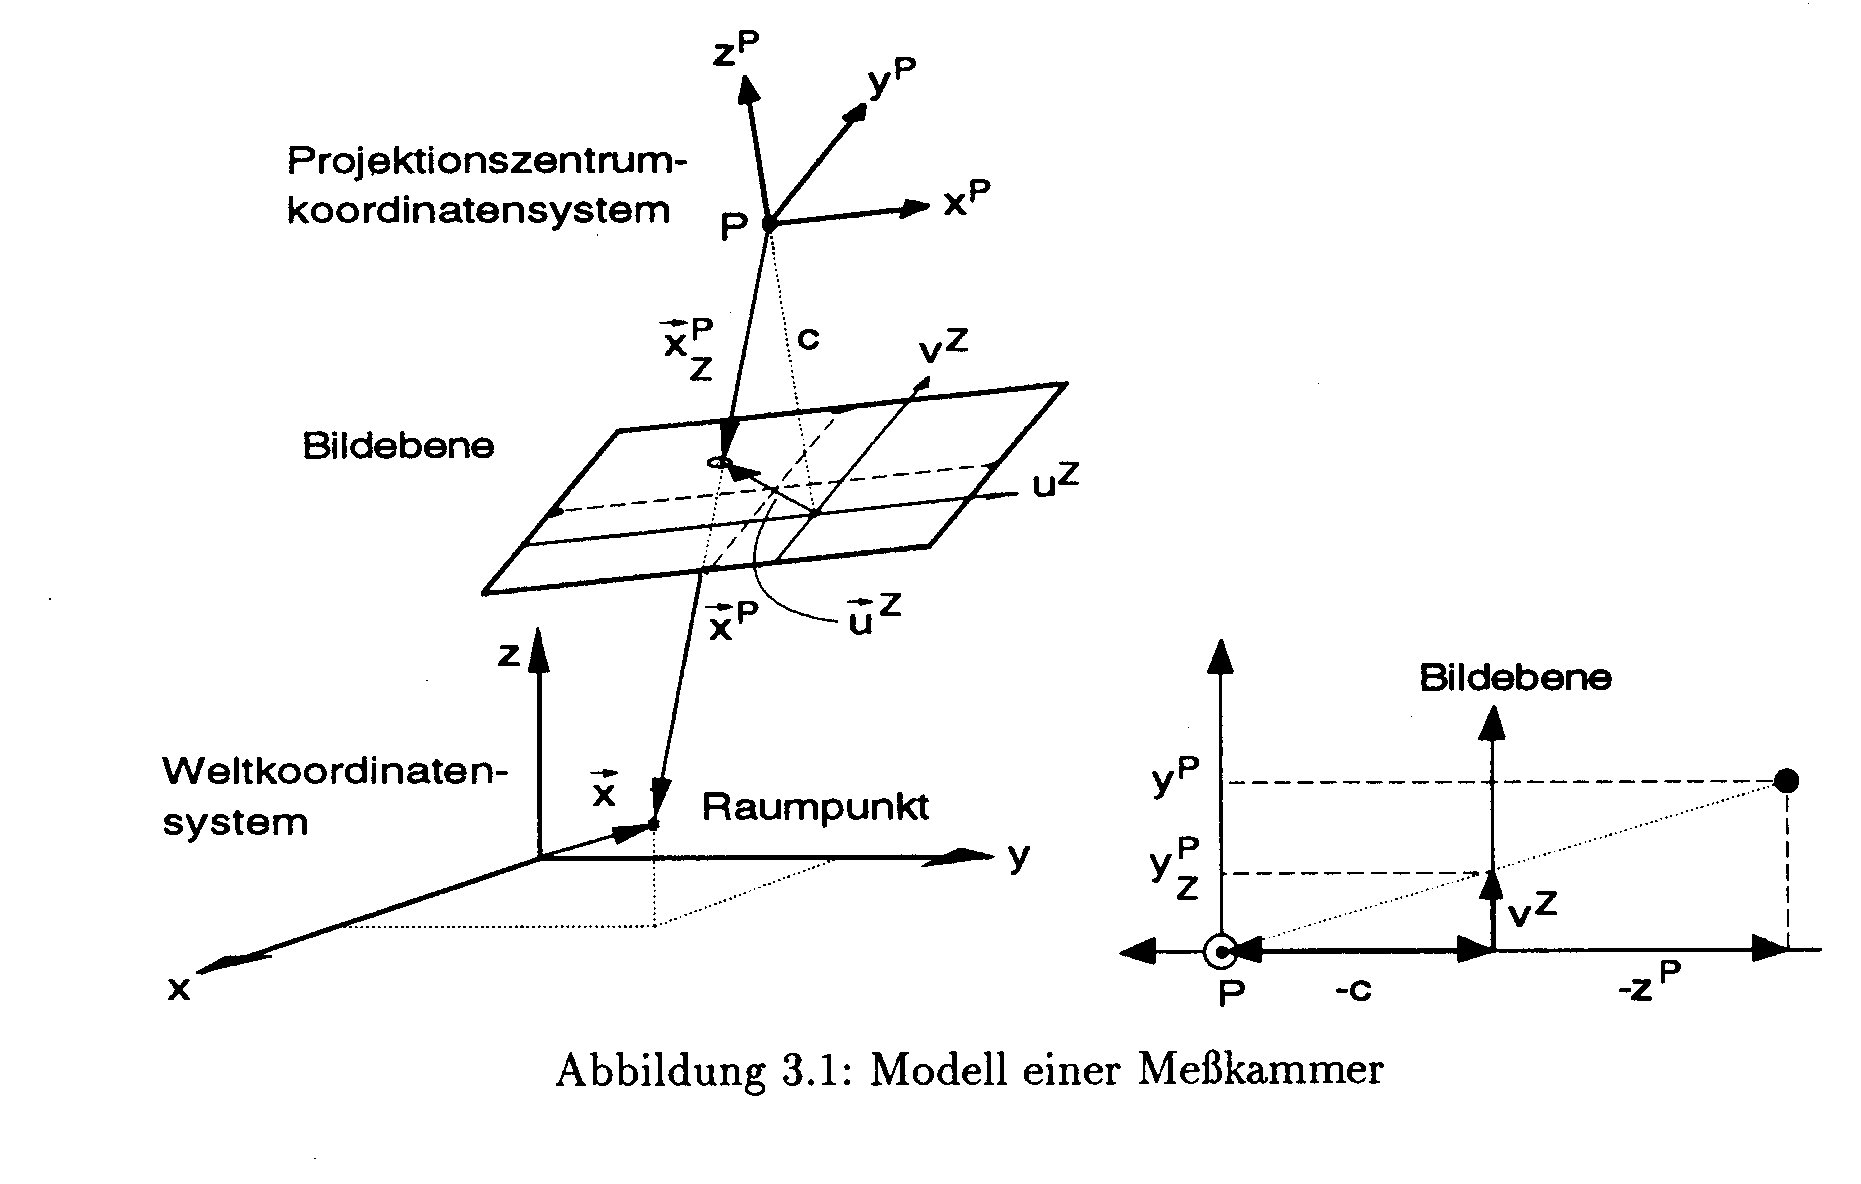
\includegraphics[width=0.65\textwidth , trim = 0mm 65mm 270mm 0mm, clip]{Bilder/cameraCalib.jpg}
			\caption{Lage des Kamerakoordinatensystems in Bezug auf Projektionsebene und Weltkoordinatensystem. \cite{Meisel:77890}}
			\label{fig:cameraCalib}
	\end{figure}

Die Kamerakalibrierung, die diesem Projekt zu Grunde liegt, ist als manuell einzustufen und kann, wenn gewünscht bzw. benötigt, zu Beginn der eigentlichen Anwendung durchgeführt werden. Um die verschiedenen Koordinatensysteme auseinander zu halten, wird zu Beginn eine Notation festgelegt, die in Tabelle~\ref{tab:camCalibParam} eingesehen werden kann. Zusätzlich können in der Tabelle sowohl die einzelnen Koordinatensysteme, als auch die einzelnen Berechnungsschritte der Kamerakalibrierung nachvollzogen werden, die im Folgenden erläutert werden. Lässt man die ersten zwei Zeilen der Tabelle weg, so ist eine Transformation von Weltkoordinaten $\overrightarrow{x}$ in Sensorkoordinaten $\overrightarrow{u}$ schematisch dargestellt. Dieses Schema muss für die Kamerkalibrierung von \textit{MaRC} invertiert werden und um die Koordinatentransformation in Unitykoordinaten ergänzt werden.  \\

\begin{table}
	\centering
	\renewcommand{\arraystretch}{1.4}
	\begin{tabular}{|c|c|c|c|}
		\hline
		\Absatzbox{}
		& \textbf{Koordinaten} & \textbf{Komponenten}&\textbf{Transformation}\\
		\hline
		$\overrightarrow{x}^U$ & Unitykoordinaten &$x^U$,$y^U$,$z^U$& \\
		\cline{2-4}
		$\downarrow$ & & & Koordinatentransformation\\
		\cline{2-4}
		$\overrightarrow{x}$ & Weltkoordinaten &$x$,$y$,$z$&  \\
		\cline{2-4}
		$\downarrow$ & & & Koordinatentransformation\\
		\cline{2-4}
		$\overrightarrow{x}^P$ & Projektionszentrumkoordinaten &$x^P$,$y^P$,$z^P$& \\
		\cline{2-4}
		$\downarrow$ & & & Projektion \\
		\cline{2-4}
		$\overrightarrow{x}^P_Z$ & Projektionszentrumkoordinaten &$u^Z$,$v^Z$,$-c$& \\
		\cline{2-4}
		$\downarrow$ & & & Linsenverzeichnung\\
		\cline{2-4}	
		$\overrightarrow{x}^P_D$ & Verzeichnungskoordinaten &$u^D$,$v^D$,$-c$& \\
		\cline{2-4}
		$\downarrow$ & & & Bildebenenverkippung\\
		\cline{2-4}		
		$\overrightarrow{x}^V$ &Verkippungskoordinaten &$u^V$,$v^V$,$-c^V$& \\
		\cline{2-4}
		$\downarrow$ & & & Bildhauptpunktverschiebung\\
		\cline{2-4}	
		$\overrightarrow{u}$ & Sensorkoordinaten &$u$,$v$ & \\
		\hline
	\end{tabular}
	\caption{Parameter und Berechnungsschritte der Kamera Kalibrierung.\cite{Meisel:77890}}
	\label{tab:camCalibParam}
\end{table}

Die einzelnen Schritte aus Tabelle~\ref{tab:camCalibParam} kann man in vier bzw. drei Abschnitte einteilen: \\
Im ersten Abschnitt wird der Hauptpunkt so versetzt, dass der Koordinatenursprung des Kamerakoordinatensystems mit dem Bildkoordinatensystem übereinstimmt. Dies geschieht, indem man für die eine Achse $u^V = u - \Delta u$ und für die andere Achse entsprechend $v^V = v - \Delta v$ berechnet.\\
Zusätzlich wird die Bildebene verkippt, so dass gilt $\overrightarrow{x}^V = R_v \cdot \overrightarrow{x}^P_D$. Bezeichnet $\varphi$ den Drehwinkel um die $x^P$-Achse und $\vartheta$ den Drehwinkel um die $y^{P'}$-Achse, so lässt sich $R_v$ wie folgt berechnen:

\begin{equation}
\label{equ:Rverkippt}
R_v = 
\begin{pmatrix}
r_{v11} & r_{v12} & r_{v13} \\
r_{v21} & r_{v22} & r_{v23} \\
r_{v31} & r_{v32} & r_{v33} \\
\end{pmatrix} = 
\begin{pmatrix}
cos\vartheta & sin\vartheta sin\varphi & -sin\vartheta cos\varphi \\
0 & cos\varphi & sin\varphi\\
sin\vartheta & -cos\vartheta sin\varphi & cos\vartheta cos\varphi \\
\end{pmatrix} 
~ ~ ~ ~ ~R_v \in \mathbb{R}^{3x3}
\end{equation}

Die negative verkippte Kamerakonstante $-c^V$, die in Tabelle~\ref{tab:camCalibParam} aufgeführt ist, berechnet sich wie in~\citep{Meisel:77890} beschrieben nach der Formel:

\begin{equation}
-c^V = - \frac{c+u^V \cdot r_{v13} + v^V \cdot r_{v23}}{r_{v33}}
\end{equation}

Im zweiten Schritt wird im Allgemeinem die Linsenverzeichnung herausgerechnet. Im vorliegenden Fall wurde bewusst auf diesen Schritt verzichtet und die zugehörigen Entzerrungskoeffizienten werden für alle weiteren Berechnungen auf null gesetzt. \textcolor{red}{Begründung??} \\

Weil wie bereits beschrieben, die Linsenverzeichnung vernachlässigt wurde, kann man Schritt 1 und 2 zu einem Schritt zusammenfassen und vereinfacht darstellen. Dieser erste Schritt, also die Hauptpunktverschiebung und Bildebenenverkippung, lässt sich mit Hilfe der intrinsischen Kameramatrix $M_{intrinsisch}$ zusammenfassen. Diese beinhaltet neben den Brennweiten $f_u$ und $f_v$ noch die Koordinaten des Hauptpunktes $u^V$ und $v^V$ in Bildkoordinaten und hat somit vier Freiheitsgrade.

\begin{equation}
\label{equ:intrinsic}
M_{intrinsisch} = 
\begin{pmatrix}
f_u & 0 & 0 & u^V \\
0 & f_v & 0 & v^V\\
0 & 0 & 1 & 0 \\
\end{pmatrix} 
~ ~ ~ ~ ~M_{intrinsisch} \in \mathbb{R}^{3x4}
\end{equation}

Zu diesem Zeitpunkt sollte nun das Kamerakoordinatensystem mit dem Weltkoordinatensystem übereinstimmen und es kann sich im nächsten Schritt darum gekümmert werden, dass das Kamerakoordinatensystem verschoben und gedreht wird. Während eine dreidimensionale Rotation im Allgemeinen mit Matrix $R$ aus Formel~\ref{equ:Rotation} beschrieben werden kann, reicht für die Translation ein Vektor, wie $t$ aus Formel~\ref{equ:Translation} aus.\

\begin{equation}
\label{equ:Rotation}
R= R_\gamma ~R_\beta ~R_\alpha =
\begin{pmatrix}
r_{11} & r_{12} & r_{13} \\
r_{21} & r_{22} & r_{23} \\
r_{31} & r_{32} & r_{33} \\
\end{pmatrix}
~ ~ ~ ~ ~R \in \mathbb{R}^{3x3}
\end{equation}



\begin{equation}
\label{equ:Translation}
t=
\begin{pmatrix}
t_x & t_y & t_z
\end{pmatrix}^T
~ ~ ~ ~ ~t \in \mathbb{R}^{3x1} 
\end{equation}

Diese beiden Transformationen können wie in Formel~\ref{equ:extrinsic} zur extrinsischen Kameramatrix $M_{etrinsisch}$ zusammengefasst werden. Diese hat sechs Freiheitsgrade, nämlich drei für den Translationsvektor $t$ und drei für die Eulerwinkel der Rotationsmatrix $R$ für die dementsprechend gelten muss $R \in SO(3)$.

\begin{equation}
\label{equ:extrinsic}
M_{extrinsisch}= 
\begin{pmatrix}
R &|& t \\
\end{pmatrix} 
~ ~ ~ ~ ~M_{extrinsisch} \in \mathbb{R}^{3x4}
\end{equation}

Schritt 1 und 2 lassen sich vereinfachen, indem man die intrinsische Kameramatrix $M_{intrinsisch}$ und die extrinsische Kameramatrix $M_{extrinisch}$ nach der Formel~\ref{equ:inAndEx} zu einer Matrix $M$ zusammenfasst.

\begin{equation}
\label{equ:inAndEx}
M = M_{intrinsisch} \cdot M_{extrinsisch}~ ~ ~ ~ ~M\in \mathbb{R}^{3x4}
\end{equation}

Die Umrechnung von Sensorkoordinaten in Weltkoordinaten kann dann mit der invertierten Matrix $M$, wie in Formel~\ref{equ:SensInWorld} berechnet werden. \

\begin{equation}
\label{equ:SensInWorld}
\overrightarrow{x} = M^{-1} \cdot \overrightarrow{u}
\end{equation}

\textcolor{red}{Umrechnung in Unitykoordinaten fehlt noch}
%SCHRITT 3:Homographie reicht nicht aus, weil nicht 2D->3D, sondern 3D nach 3D --> Affine Transformation

%Entsprechend Formel~\ref{equ:SensInWorld} muss eine Transformationsmatrix von Weltkoordinaten in Unitykoordinaten gefunden werden. 



\subsubsection{Kalibrierung des Arbeitsbereichs}\label{sec:planeCalib} \todo[inline]{Laura}
\subsubsection{Kalibrierungfehler} \label{sec:calibError}\todo[inline]{Laura}
\subsubsection{Mögliche Fehlerquellen} \label{sec:calibErrorSources}\todo[inline]{Laura}



